\section{Introduction}
\label{sec:intro}
The standard model (SM) has been extremely successful at describing particle physics phenomena for decades. Despite its success,
the SM suffers from such shortcomings as the hierarchy problem, where fine-tuned cancellations of large quantum corrections to the Higgs
boson mass are required in order for it to be at the electroweak scale. Therefore, the recent discovery of a Higgs boson completes the
quest for the SM and yet opens a new horizon in particle physics.

Supersymmetry (SUSY) is an attractive extention to the SM, which is based on a new symmetry between bosons and fermions. It
predicts the existence of a superpartner for every SM particle, with the same quantum numbers but differing by one half unit of spin.
In R-parity conserving SUSY models, supersymmetric particles are created in pairs, and the lightest supersymmetric particle (LSP)
is stable.

The leading divergent contribution to the Higgs boson mass from SM particles arises from the Higgs boson coupling to the top quark.
SUSY provides a possible way to stabilize it through the addition of contributions from a scalar top quark. Furthermore, it offers a
number of other attractive features, such as unification of the gauge couplings and dark matter particle candidate (via the stable LSP).
The relatively low Higgs boson mass of about 125 \GeV implies that light scalar top quark with a mass
in the hundreds of GeV range is preferred in SUSY. In light of this, searches for strong production of top squark pairs have gained strong
prominence.

In this note we present the result of a search for top squark pair production in events with single isolated charged lepton (electron or muon),
jets and significant transverse momentum imbalance. The search was performed on a dataset corresponding to an integrated luminosity of 2.3\fbinv
of proton-proton (pp) collisions collected at a center-of-mass energy of 13 TeV with the Compact Muon Solenoid (CMS) detctor at the LHC.
Similar searches were previously reported by the ATLAS and CMS collaborations using datasets of 8 TeV pp collisions and by the CDF
and D0 collaborations at the Tevatron. No excess above Standard Model (SM) expectations was observed and the results of these searches were
used to place lower limits on the masses of pair produced top squarks for different decay scenarios. Depending on the decay mode, the results
probed top squarks with masses in the range of approximately $90-700$\GeV. For small neutralino masses, top squark masses up to 700\GeV were
excluded at a 95\% confidence level.

With the increase of the LHC collision energy from 8 to 13 TeV, the signal cross-section rises by a factor of 8--12 for top
squarks in mass range $700-1000$\GeV. Therefore, even with smaller 13 TeV dataset, the search has the potential to surpass sensitivity
of LHC Run 1 to top squark pair production.

The search presented here focuses on the three processes of interest:
\begin{subequations}
\begin{align}
\label{sgnProc}
pp\rightarrow\tilde{t_1}\tilde{t_1}^*\rightarrow t^{(*)}\bar{t}^{(*)}\chi^0_1\chi^0_1, \\
pp\rightarrow\tilde{t_1}\tilde{t_1}^*\rightarrow b\bar{b}\chi^+_1\chi^-_1 \rightarrow b\bar{b}W^{+(*)}W^{-(*)} \chi^0_1\chi^0_1,\\
pp\rightarrow\tilde{t_1}\tilde{t_1}^*\rightarrow t^{(*)}\chi^0_1b\chi^+_1,
\end{align}
\end{subequations}
as illustrated in Figure~\ref{fig:diagram} with one of the $W$ bosons decaying leptonically.
Here the neutralinos ($\chi^0_1$) and charginos ($\chi^+_1$) are mixtures of the superpartners
of electroweak gauge bosons and the Higgs boson. The lightest neutralino $\chi^0_1$ is often considered to be the LSP
which escapes without detection and results in large imbalance in transverse momentum. The main backgrounds in the single lepton
topology are semi-leptonic decays of \ttbar and \wjets. While the first two processes (1a and 1b) have
already been searched for during Run-1, the mixed decay mode (1c) is being explored with dedicated search regions for the first time.
Under the hypothesis of almost degenerated $\tilde{t}_{1}$ and $\chi_{1}^{0}$, this process can be observed in a final state with an
isolated lepton, two bottom quarks and transverse momentum imbalance.
\begin{figure}[!htpb]
\centering
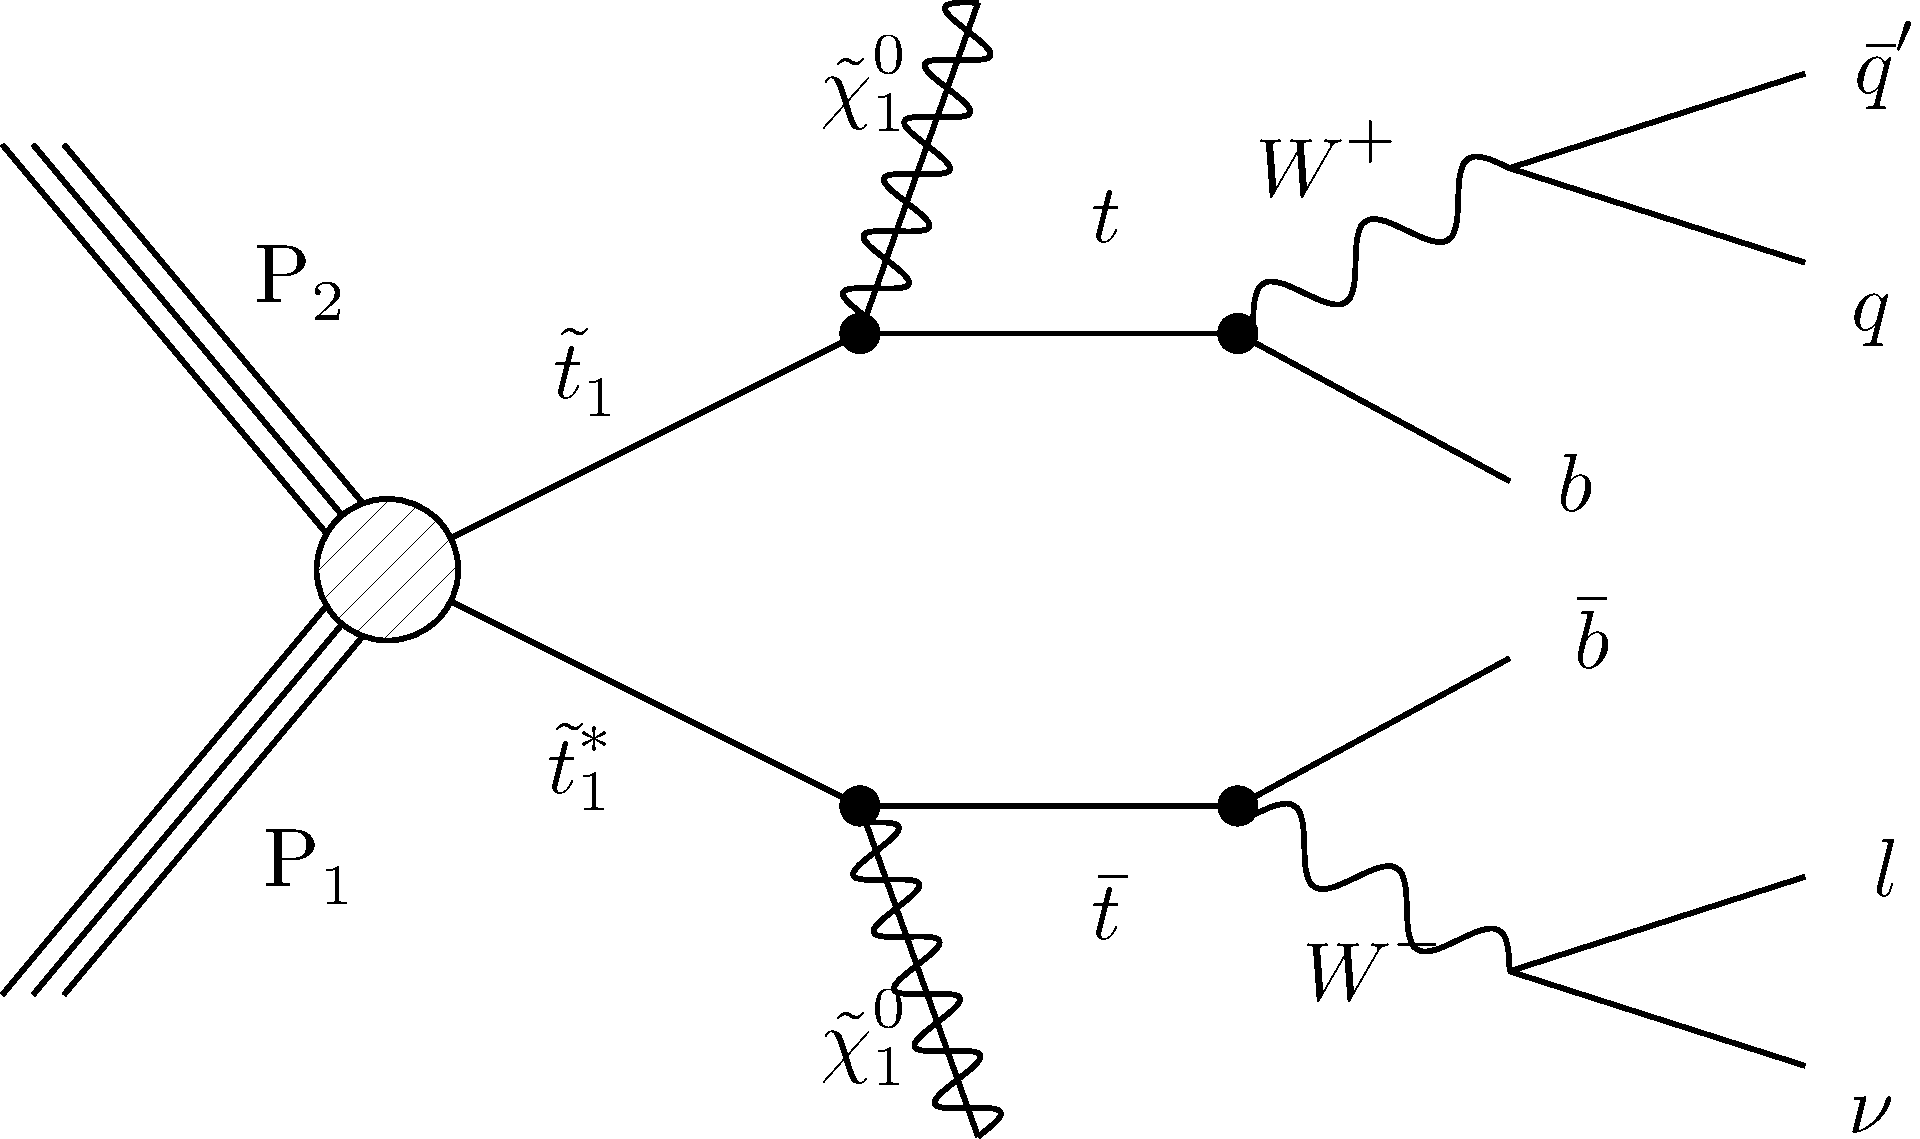
\includegraphics[width=0.45\linewidth]{plots_stop/T2tt1l_feyn.pdf}
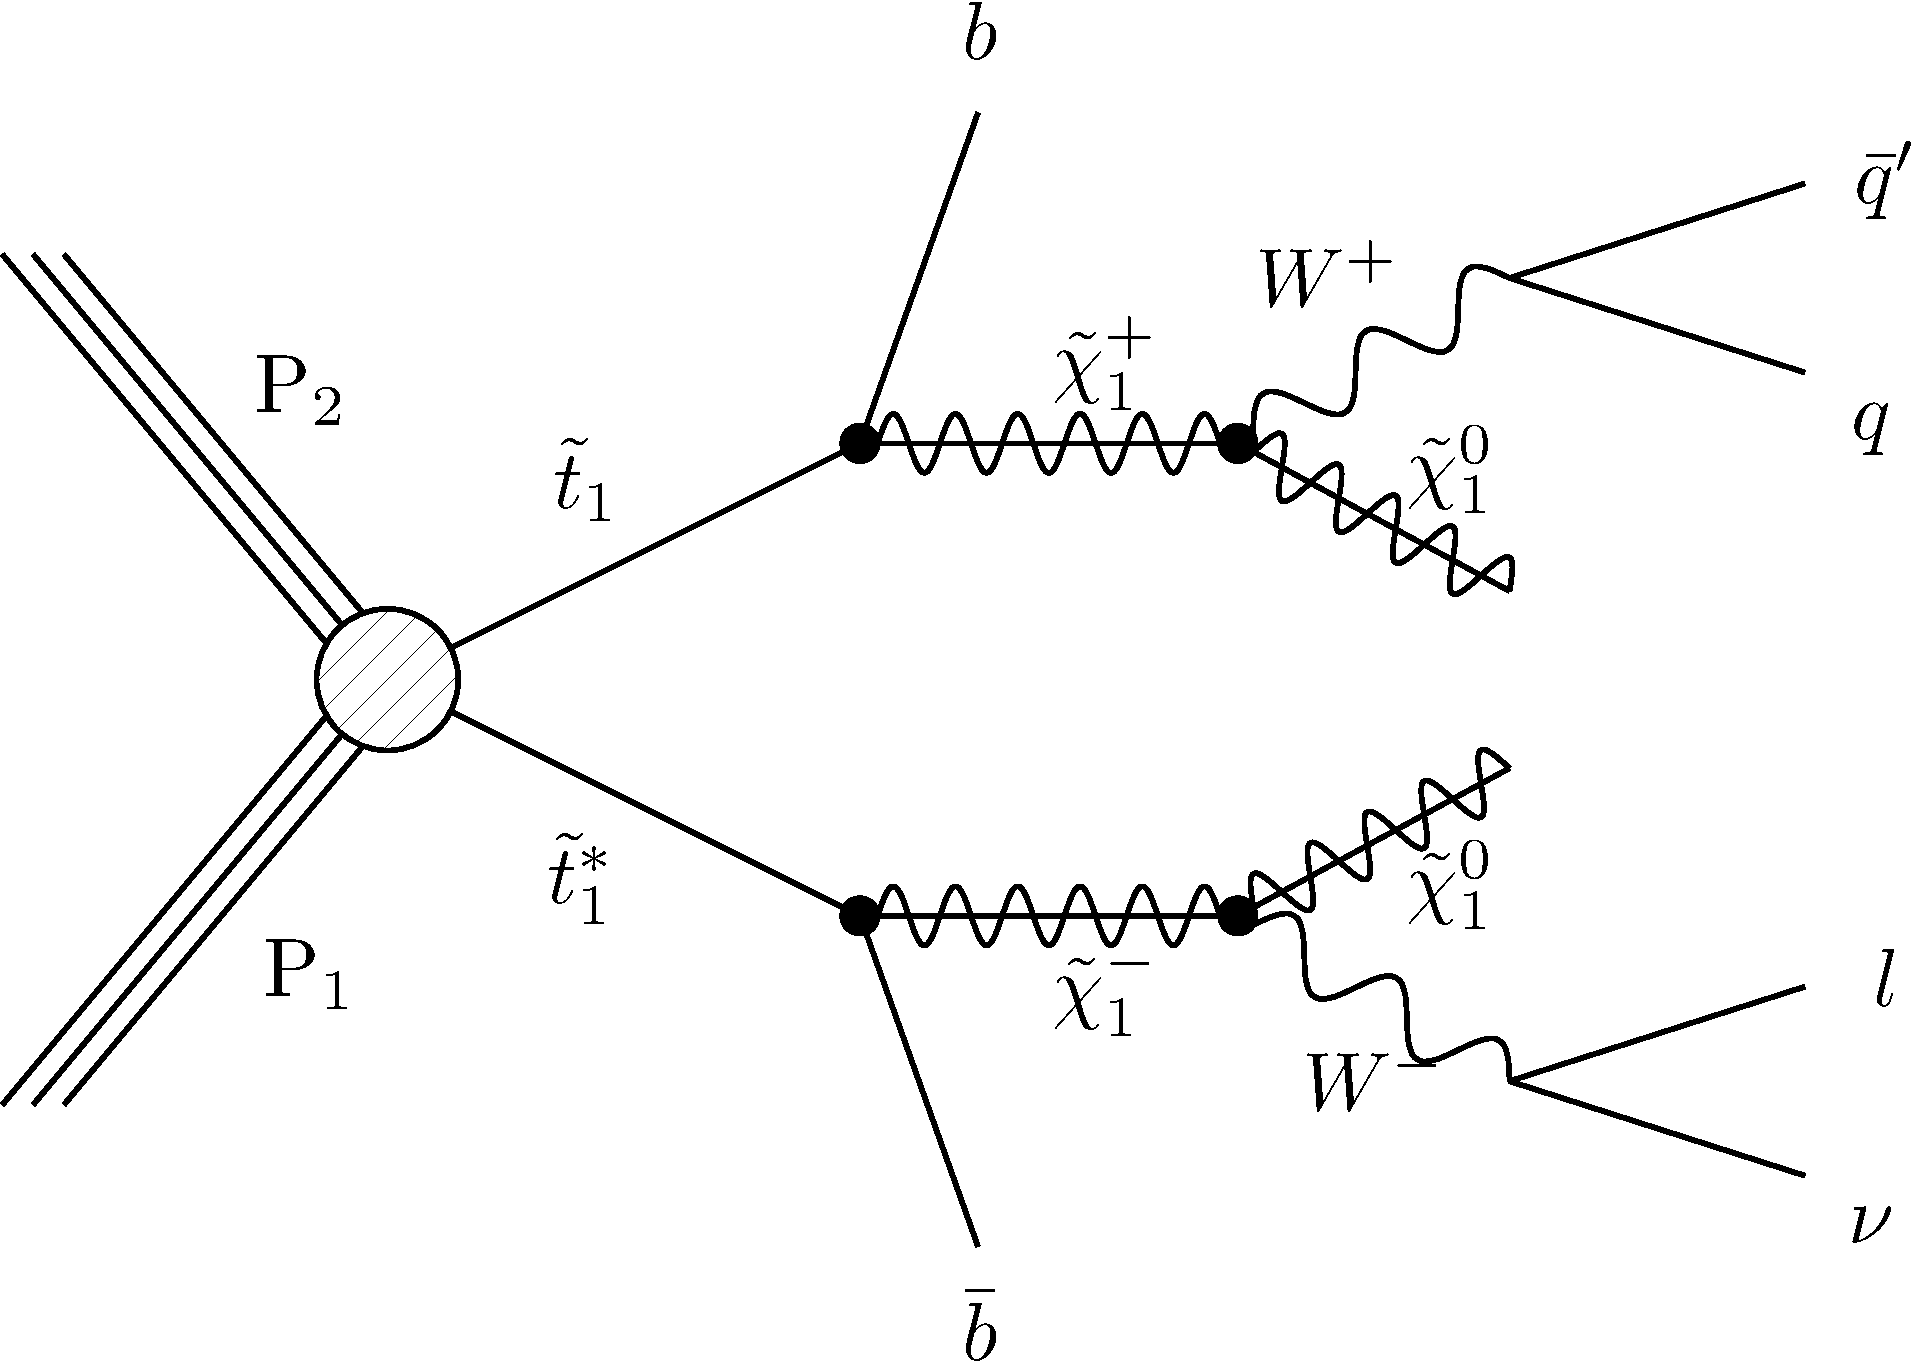
\includegraphics[width=0.45\linewidth]{plots_stop/T2bW1l_feyn.pdf}
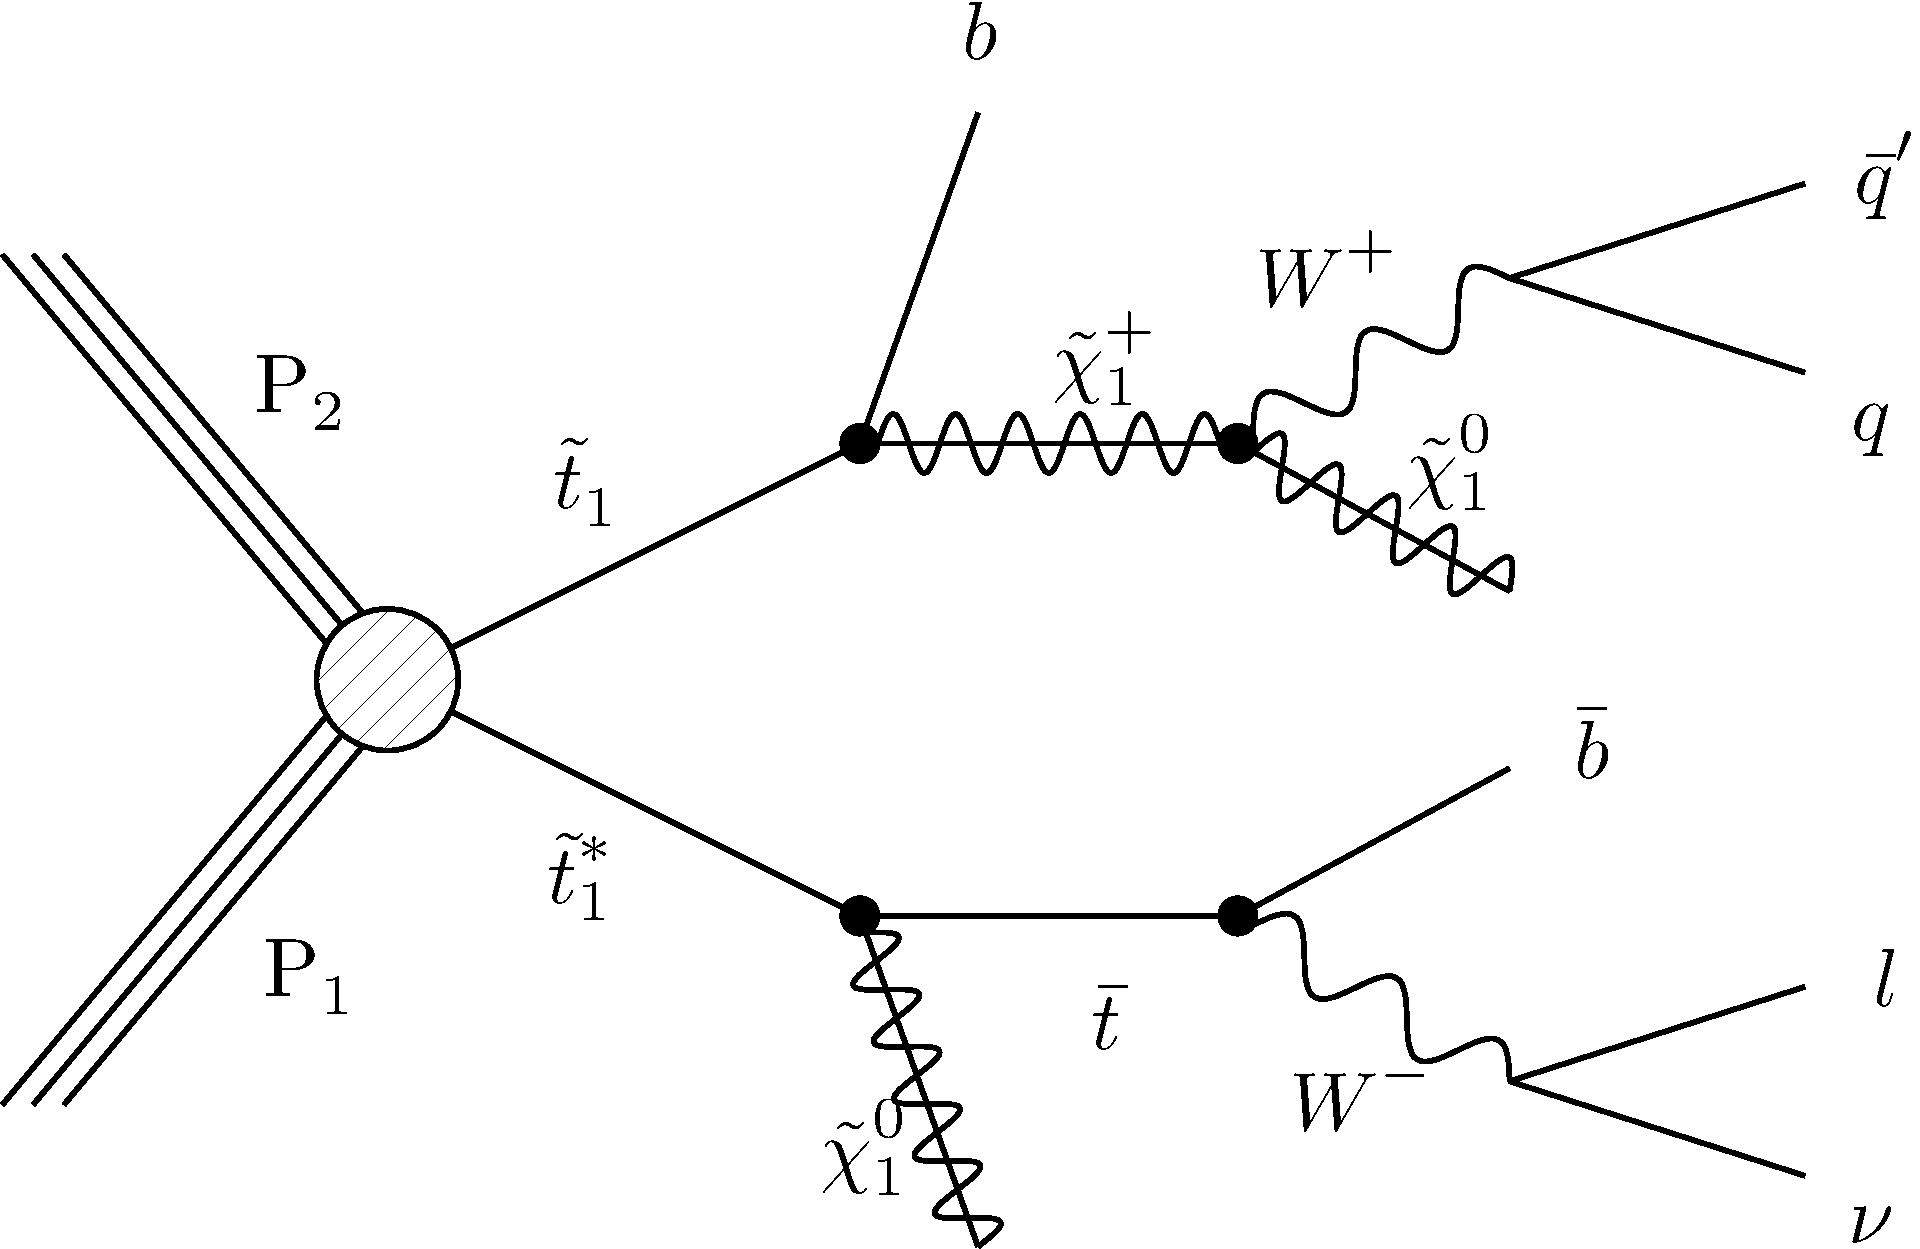
\includegraphics[width=0.45\linewidth]{plots_stop/T2tb1l_feyn.pdf}
\label{sgnProc}
\caption{
  \label{fig:diagram}
        Diagrams for the top squark pair production corresponding to different decay modes shown in Eq.~(1a), (1b), and (1c).}
\end{figure}

